\documentclass[10pt]{article}
% Midterm report (11-785). Same layout as main.tex (NeurIPS-like 5.5 x 9 in text block, Times).
% If the course Overleaf template differs, paste the sections below into it unchanged.
\usepackage[letterpaper,textwidth=5.5in,textheight=9in,top=1in,headheight=12pt,headsep=25pt,footskip=30pt]{geometry}
\usepackage[T1]{fontenc}
\usepackage[utf8]{inputenc}
\usepackage{mathptmx}
\usepackage{amsmath,amssymb}
\usepackage{microtype}
\usepackage{booktabs}
\usepackage{graphicx}
\usepackage{xcolor}
\usepackage[numbers,sort&compress]{natbib}
\usepackage[small,labelfont=bf]{caption}
\usepackage{enumitem}
\usepackage{multirow}
\usepackage{tabularx}
\usepackage[colorlinks=true,linkcolor=blue!50!black,citecolor=blue!50!black,urlcolor=blue!50!black]{hyperref}
\setlist{nosep,leftmargin=1.4em}
\setlength{\textfloatsep}{8pt plus 2pt minus 2pt}
\setlength{\floatsep}{8pt plus 2pt minus 2pt}
\renewcommand{\topfraction}{0.92}
\renewcommand{\bottomfraction}{0.6}
\renewcommand{\textfraction}{0.08}
\renewcommand{\floatpagefraction}{0.85}
\setcounter{topnumber}{3}

\newcommand{\repo}{\url{https://github.com/chilalaabubakar/IDL-PROJECT}}
\newcommand{\Dm}{D1$^{-}$}
\newcommand{\Dp}{D1$^{+}$}
\newcommand{\pmsd}[2]{#1\,{\scriptsize$\pm$\,#2}}
\newcommand{\fillin}[1]{\textcolor{red}{[#1]}}

\title{Placing Defects Where You Ask:\\ Generating Defects at Chosen Sites in a Model Glass\\ with a Diffusion Model\\[4pt] \large Midterm report}

\author{
  Stacy Cheruto \quad Nicholaus Ladislaus \quad Abubakar Chilala\\ Gentille Uwera \quad Michel Sangwa \quad Boniface Godwin\\[2pt]
  College of Engineering, Carnegie Mellon University Africa\\
  {\small\texttt{\{ccheruto, eladisla, achilala, guwera, sbmichel, bgodwin\}@andrew.cmu.edu}}
}
\date{}

\begin{document}
\maketitle

\begin{abstract}
Defects, small groups of atoms arranged differently from the rest, control how a glass breaks, ages or absorbs light, and studying one needs many realistic copies of it. Today researchers wait for it to form in slow melt-and-cool simulations or insert it by hand, which can leave unnatural surroundings. We train a diffusion model that rebuilds a small region around a chosen site inside an existing glass and is told which defect to create there. On a two-dimensional model glass, over three training runs, it places under-coordinated atoms 3.5 times as often as hand insertion (0.22 vs.\ 0.06) and B-rich defects 1.5--2.4 times as often (0.45--0.71 vs.\ 0.30), with atom energies closer to those around natural defects. New since the draft: choosing the guidance strength for each trained model halves the spread between training runs; the rebuilt region leaves a seam at its edge; and placed defects survive heating slightly less often than natural ones.
\end{abstract}

\section{Introduction: motivation and objectives}

Glasses have no regular crystal lattice, but they still contain defects, and how a defect behaves depends on the atoms around it. Studies of how glasses deform, age or absorb light therefore need many realistic examples of the same defect at chosen places. In a melt-and-cool (melt-quench) molecular dynamics (MD) simulation one waits for the defect to form by chance, which is slow for rare defects; in hand insertion atoms are moved by hand and relaxed, which is fast but can leave unnatural surroundings. Diffusion models such as DM2~\citep{yang2026dm2} generate realistic glasses but are controlled by whole-sample properties such as the cooling rate, not by a defect at a place. 

Like image inpainting~\citep{lugmayr2022repaint}, the model fills in a region cut out of an existing glass (the rest held fixed) and is told which defect to put at its centre (Task~B, Figure~\ref{fig:overview}). Our objectives:
\begin{enumerate}
\item[\textbf{O1}] \textbf{Placement:} after relaxation, the requested defect is at the site in more of 256 requests than with hand insertion or local melt-quench.
\item[\textbf{O2}] \textbf{Realism:} atom energies around a placed defect are close to those around natural defects (local W1 near the natural floor, below hand insertion).
\item[\textbf{O3}] \textbf{Reliability:} O1 and O2 hold over three training runs and under changes to the evaluation settings.
\end{enumerate}
We use a two-dimensional model glass, where every step is cheap enough to check carefully, before moving to three-dimensional silica (Section~\ref{sec:next}).

\begin{figure}[t]
\centering
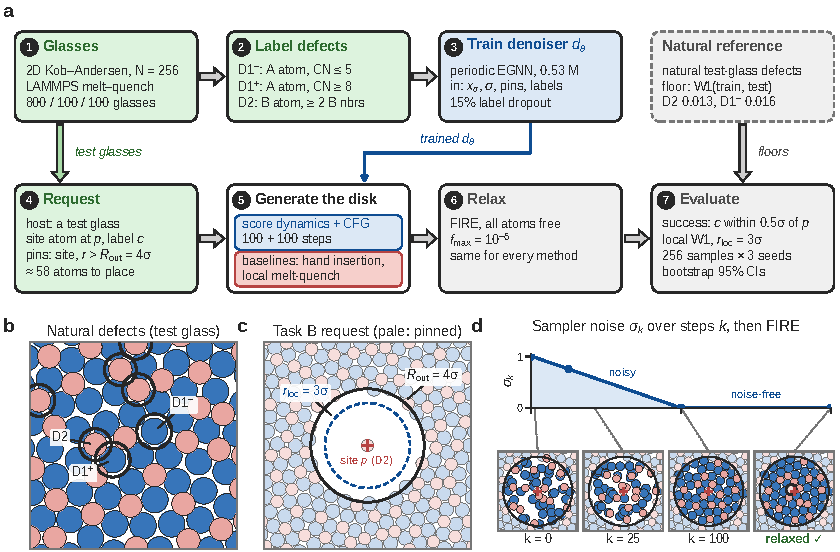
\includegraphics[width=0.8\linewidth]{figures/fig1_overview.pdf}
\caption{Overview. \textbf{(a)} Workflow: make glasses by melting and cooling (1), label their defects (2), train the network (3); a request (4) names a glass, a site and a defect type; the model or a baseline fills the region (5); every result is relaxed with all atoms free (6) and scored (7). \textbf{(b)} Natural defects (rings) in a test glass; large blue atoms are type A, small pink atoms type B. \textbf{(c)} A real request: pale atoms are held fixed, including the atom at the site; atoms inside the solid circle ($R_\text{out}$) are rebuilt; the dashed circle ($r_\text{loc}$) is the area used to judge realism. \textbf{(d)} The model filling this region: atoms start at random positions and are cleaned up as the noise level falls; after relaxation the requested D2 defect sits at the site.}
\label{fig:overview}
\end{figure}

\section{Related work and background}

\textbf{Diffusion models for materials.} Diffusion models~\citep{ho2020ddpm,song2021sde} turn noise into data step by step and now generate crystals~\citep{xie2022cdvae,jiao2023diffcsp,zeni2025mattergen} and glasses. Our starting point is \textbf{DM2}~\citep{yang2026dm2}: a network learns to predict random shifts added to atom positions, and new glasses are built by repeating this clean-up with small random kicks (score dynamics). We keep its training target and sampler, use an unlabelled model like DM2's as the ``chance'' baseline, and follow DM2 in judging realism by comparing structural distributions with MD-made glasses; our local W1 does this around one defect. Other work steers whole samples with spectra or target properties~\citep{kwon2024spectroscopy,finkler2026inverse}.

\textbf{Local control.} RePaint~\citep{lugmayr2022repaint} fills a masked image region (our Task~A baseline); classifier-free guidance~\citep{ho2022cfg} makes a model follow a label more strongly. In materials, the closest work fills in crystals around a fixed host~\citep{zhong2025inpainting} or relaxes crystals with point defects~\citep{cui2026constrained}; glasses have no lattice to compare with, so realism must be judged against many natural examples.

\section{Data and methods}

\textbf{Dataset.} We generate our own data with LAMMPS~\citep{thompson2022lammps}, using the two-dimensional Kob--Andersen glass~\citep{kob1995,bruning2009}: two atom types, A (large, 65\%) and B (small, 35\%), interacting through Lennard-Jones forces, in a periodic square box; $\sigma$, the size of an A atom, is the unit of length. Preparation: random placement, melt at $T=2.0$ for 100 time units, cool by $10^{-2}$ per time unit to $T=0.01$, minimise the energy, reject glasses that crystallise or contain overlapping atoms or outlier energies, and label defects with rules fixed on the training glasses. The main set has 800/100/100 train/validation/test glasses of $N=256$ atoms (box side $14.6\sigma$); 1600/200/200 glasses with $N=64$ serve a symmetry test. An atom's neighbours are the atoms within 1.4 times the contact distance. \Dm{} is an A atom with at most 5 neighbours (1.7 per glass), \Dp{} an A atom with at least 8 (1.4 per glass), and D2 a B atom with at least two B neighbours within $1.2\sigma$ (10 per glass). A library of 10,545 natural defects with their neighbourhoods, cut from the training glasses, supplies hand insertion.



\textbf{Model.} The network $d_\theta(x_\sigma,\sigma,m,c)$ takes noisy atom positions $x_\sigma$, the noise level $\sigma$, a held-fixed flag $m_i$ and a label $c_i$ for each atom (``none'' everywhere except the site), and returns one 2D arrow per atom: its estimate of how far noise has moved that atom (Figure~\ref{fig:arch}). Shifting, rotating or renumbering a glass should do the same to the arrows, so we use an E($n$)-equivariant graph neural network (EGNN)~\citep{satorras2021egnn} adapted to periodic boxes: atoms within $2.5\sigma$ are linked, messages depend only on distances, and each output arrow is a weighted sum of neighbour vectors (zero on held atoms). Table~\ref{tab:models} lists the models and their settings.

\begin{figure}[t]
\centering
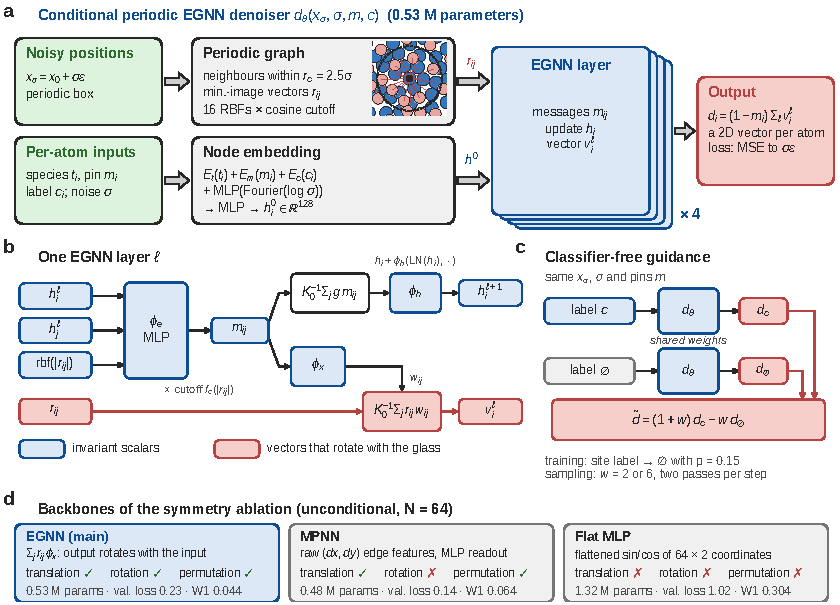
\includegraphics[width=0.8\linewidth]{figures/fig2_architecture.pdf}
\caption{The networks. \textbf{(a)} The conditional denoiser: noisy positions define a periodic graph, per-atom inputs define starting features, and four EGNN layers turn both into one arrow per atom. \textbf{(b)} One EGNN layer: blue items do not change when the glass is rotated; red items rotate with it. \textbf{(c)} Classifier-free guidance runs the same network with and without the site label. \textbf{(d)} The three networks of the symmetry test.}
\label{fig:arch}
\end{figure}

\begin{table}[t]
\centering
\caption{Model description. All models train with AdamW (learning rate $2\times10^{-4}$, batch 16, gradient clipping 1, weight moving average 0.999), 50,000 updates with labels or 40,000 without; one run takes about 4 hours on a T4 GPU. Sampling: 100 noisy plus 100 noise-free steps.}
\label{tab:models}
\small
\begin{tabularx}{\linewidth}{@{}l>{\raggedright\arraybackslash}X>{\raggedright\arraybackslash}Xr@{}}
\toprule
Model & Layers & Settings tried & Params \\
\midrule
EGNN (main) & 4 EGNN layers, 128 features, 16 radial basis functions, cutoff $2.5\sigma$ & $\sigma_\text{max}\in\{0.5,1.0\}$; $R_\text{out}=4\sigma$ or 3--6$\sigma$; guidance $w=0$--8; seeds 0--2 & 0.53\,M \\
MPNN & same graph, raw $(dx,dy)$ edges, MLP read-out & $N=64$, no label & 0.48\,M \\
Flat MLP & 4 layers of 512 units on sorted coordinates & $N=64$, no label & 1.32\,M \\
\bottomrule
\end{tabularx}
\end{table}

\textbf{Loss.} Following DM2, noise is added to the free atoms, $x_\sigma=x_0+\sigma\varepsilon$ with $\varepsilon\sim\mathcal N(0,I)$ and $\sigma\sim\mathcal U(10^{-3},\sigma_\text{max})$, and the network predicts the added shift. The loss is the mean squared error over the free atoms $U$: $\mathcal L=\mathbb E\big[\tfrac{1}{|U|}\sum_{i\in U}\lVert d_\theta(x_\sigma,\sigma,m,c)_i-\sigma\varepsilon_i\rVert^2\big]$. Training requests are whole boxes (50\%), small patches (30\%) or filled-in regions (20\%), centred on a natural defect half of the time; the label is hidden 15\% of the time, which classifier-free guidance needs. Sampling combines the predictions with and without the label, $\tilde d=(1+w)\,d_\theta(\cdot,c)-w\,d_\theta(\cdot,\varnothing)$.

\textbf{Baselines (implemented in our pipeline).} \emph{Chance}: fill the region with no label (DM2-style), showing how often the defect appears anyway. \emph{Hand insertion}, the common practice: paste a natural defect and its neighbours within $1.5\sigma$ from a training glass at the site. \emph{Local melt-quench}, the MD way: freeze the atoms beyond $R_\text{out}$, then melt and cool the region in LAMMPS. Task~A (a whole new box) adds clamping and RePaint~\citep{lugmayr2022repaint}. All methods answer the same 256 requests.

\textbf{Evaluation metrics.}\label{sec:metrics}
\emph{Success}: after relaxation with the FIRE algorithm~\citep{bitzek2006fire} (all atoms free, largest force below $10^{-6}$), the atom of the requested type nearest the site lies within $0.5\sigma$ of it and carries the requested label. This is the quantity a user cares about.
\emph{Local W1}: the Wasserstein-1 distance between the energies of atoms within $r_\text{loc}=3\sigma$ of the site and the same energies around natural defects of that type in the test glasses. Lower means closer to natural; natural training-glass defects against test-glass defects give the \emph{natural floor} (D2 0.013, \Dm{} 0.016). We report 95\% bootstrap confidence intervals over the 256 samples.

\section{Experiments and results}

\textbf{Iterations so far.} We trained 13 models, all to completion: two without labels (the chance baseline), three conditional models per noise range and seed (seeds 0--2 for $\sigma_\text{max}=0.5$, used for \Dm{}, \Dp{} and Task~A, and for $\sigma_\text{max}=1.0$, used for D2), three networks for the symmetry test at $N=64$, and two conditional models trained on a range of region sizes. The first conditional model used DM2's noise range ($\sigma_\text{max}=0.5$), but sampling starts at $\sigma=1$, a level the network had never seen; retraining with $\sigma_\text{max}=1.0$ raised D2 success from 0.54 to 0.79 (seed 0, $w=6$). We cut the sampler from DM2's 2,900 steps to 100: longer runs over-cool the glass at 15 times the cost.

\textbf{Main result and baseline evidence.} Table~\ref{tab:main} gives Task~B over 256 requests per run. Every baseline row comes from our own code on the same requests; we also re-ran DM2's published silica model and confirmed its local structure (99.3\% of Si atoms with four O neighbours). The model beats both baselines for D2 and \Dm{} (O1). At $w=2$ its \Dm{} surroundings score 1.2--1.5 times the natural floor and its D2 surroundings 0.045--0.056 against 0.087 for hand insertion (O2). Local melt-quench almost never creates the defect: re-melting a 60-atom region is waiting on a small scale. No method places \Dp{}: a natural \Dp{} moved into another glass with its 47 nearest atoms disappears on relaxation 97\% of the time, so what holds it lies further away. The ranking of methods held when we moved the defect rules, success radius, realism window or region size, and re-runs with the same seed reproduced 8 of 9 rows exactly (O3).

\begin{table}[t]
\centering
\caption{Task~B: success after relaxation and local W1 (lower is closer to natural). Model rows: mean $\pm$ standard deviation over three training runs; baselines: estimate with 95\% CI. D2 uses $\sigma_\text{max}=1.0$; \Dm{} and \Dp{} use $\sigma_\text{max}=0.5$. $^\dagger$2,900-step sampler. $^\ddagger$Seed 0 only. $^\S$New since the draft: $w$ chosen per model on validation glasses (Section~\ref{sec:new}).}
\label{tab:main}
\small
\setlength{\tabcolsep}{4pt}
\begin{tabular}{@{}lccccc@{}}
\toprule
& \multicolumn{2}{c}{D2 (B-rich)} & \multicolumn{2}{c}{\Dm{} (too few neighbours)} & \Dp{} \\
\cmidrule(lr){2-3}\cmidrule(lr){4-5}\cmidrule(l){6-6}
Method & success & local W1 & success & local W1 & success \\
\midrule
Chance (no label)$^\dagger$ & 0.03 & 0.062 & 0.02 & 0.053 & 0.00 \\
Local melt-quench & 0.05 {\scriptsize[0.03, 0.08]} & 0.065 & 0.00 {\scriptsize[0.00, 0.00]} & 0.024 & 0.01 \\
Hand insertion & 0.30 {\scriptsize[0.24, 0.36]} & 0.087 & 0.06 {\scriptsize[0.04, 0.09]} & 0.032 & 0.02 \\
\midrule
Model, $w=2$ & \pmsd{0.45}{0.11} & \textbf{\pmsd{0.051}{0.006}} & \textbf{\pmsd{0.22}{0.02}} & \textbf{\pmsd{0.022}{0.002}} & 0.03$^\ddagger$ \\
Model, $w=6$ & \pmsd{0.71}{0.08} & \pmsd{0.072}{0.016} & \pmsd{0.21}{0.04} & \pmsd{0.038}{0.004} & 0.04$^\ddagger$ \\
Model, $w$ per model$^\S$ & \textbf{\pmsd{0.74}{0.04}} & \pmsd{0.076}{0.013} & --- & --- & --- \\
\midrule
Natural floor & --- & 0.013 & --- & 0.016 & --- \\
\bottomrule
\end{tabular}
\end{table}



\subsection{New experiments since the draft}
\label{sec:new}

\begin{figure}[t]
\centering
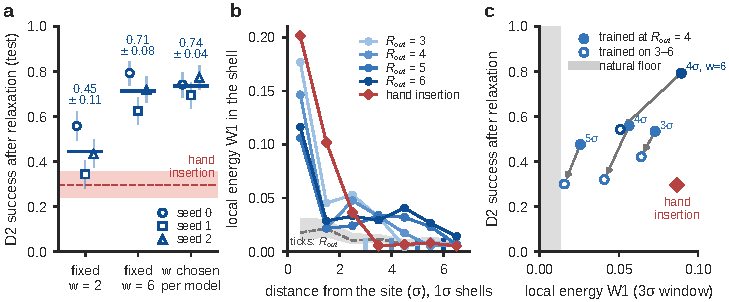
\includegraphics[width=\linewidth]{figures/fig6_followups.pdf}
\caption{Follow-up checks (Task~B, D2). \textbf{(a)}~Test success for the three training runs at fixed $w$ and at the $w$ each model's validation rows chose (target: validation success $\ge0.70$; chosen $w=4, 8, 8$). The bar is the mean; the red band is hand insertion. \textbf{(b)}~Local energy W1 in $1\sigma$ shells around the site for regions of radius $R_\text{out}=3$--$6\sigma$ (seed 0, $w=2$), hand insertion, and the natural floor (grey); ticks on the axis mark each $R_\text{out}$. \textbf{(c)}~Success against local W1 for the model trained at $R_\text{out}=4\sigma$ (filled) and the model trained on 3--6$\sigma$ (open), at the same sampling settings (labels give $R_\text{out}$; dark: $w=6$, light: $w=2$).}
\label{fig:followups}
\end{figure}

\textbf{Choosing $w$ for each model.} The three D2 runs follow the label with different strength although their validation losses agree within a few percent. We sampled each at $w=1$--$8$ on \emph{validation} glasses and applied rules fixed beforehand. The success rule (smallest $w$ with validation success $\ge0.70$) chose $w=4, 8, 8$; on the test glasses this gives 0.74 $\pm$ 0.04, half the spread of fixed $w=6$ (0.71 $\pm$ 0.08), with similar local W1 (Figure~\ref{fig:followups}a). The realism rule (local W1 $\le0.07$) chose $w=2$ for every model and changed nothing, because validation W1 runs higher than test W1.

\textbf{A seam at the edge of the rebuilt region.} A region of $R_\text{out}=5\sigma$ had given much lower local W1 than $4\sigma$ (0.026 vs.\ 0.056). Shell by shell (Figure~\ref{fig:followups}b), the mismatch is largest at the defect, stays at about 3 times the floor up to the edge of the rebuilt region, and reaches the floor about $1\sigma$ beyond it; hand insertion damages only the first $3\sigma$. A larger region lowers the mismatch near the site, but over a $6\sigma$ window every region size scores about the same (W1 0.024--0.026, hand insertion 0.022), so part of the earlier gain was the seam moving out of the $3\sigma$ window.

\textbf{Training on a range of region sizes.} Drawing $R_\text{out}$ from 3--6$\sigma$ during training left \Dm{} unchanged (0.16--0.22 vs.\ 0.18--0.25). The D2 model, with equal validation loss, followed the label more weakly: fewer successes (0.30--0.54 vs.\ 0.48--0.79), lower W1 (0.016--0.064 vs.\ 0.026--0.089; Figure~\ref{fig:followups}c): along the trade-off, not beyond.

\textbf{\Dp{} with a larger region.} Rebuilding $5$--$6\sigma$ instead of $4\sigma$ does not help (success 0.03--0.05): the defect is placed in 24--43\% of samples but lost on relaxation.

\textbf{Physical checks.} Table~\ref{tab:main} pools failed and successful requests. Successful D2 placements alone ($R_\text{out}=6\sigma$, $w=2$, seed 0) have local W1 0.029 (natural 0.012, hand insertion 0.094). Host atoms $6$--$7\sigma$ away move by $0.180\sigma$ on relaxation (hand insertion $0.064\sigma$). In free MD (56 hosts, three runs each) the defect remains after 250 time units in 87\% of generated, 91\% of hand-inserted and 95\% of natural cases at the dataset's final temperature. Over all 256 requests, 0.48, 0.26 and 0.34 (three runs) end with the defect placed and still present (hand insertion 0.27, no label 0.11).

\section{Discussion: challenges and risks}

The model meets O1 and O3 for two of three defect types, with lower pooled local W1 than hand insertion (O2). Challenges: runs with equal loss follow the label differently (we now choose $w$ per model); the host is disturbed up to the region's edge and placed defects are a little less stable than natural ones; \Dp{} needs more than a larger region. The main risk is 3D silica: about 1\,s per training update, 565 CPU core-hours of MD, and rare defects (well under one per glass).

\section{Next steps}
\label{sec:next}
\begin{enumerate}
\item \textbf{Finish generalisation} (week 10). On fresh glasses of the training kind the runs place D2 in 0.51, 0.36, 0.43 of requests (hand insertion 0.23); 1,024-atom glasses and 10$\times$ slower or faster cooling are running.
\item \textbf{Start 3D silica} (weeks 9--13): train our conditional NequIP~\citep{batzner2022nequip} on DM2's 24 glasses (code ready) and make 576-atom glasses with DM2's potential~\citep{bouhadja2013}, targeting wrongly coordinated Si, non-bridging oxygens and 3-rings.
\item \textbf{Fix the weaknesses}: choose $w$ per model by default, anneal the seam shell after sampling, and give \Dp{} a label for its wider surroundings.
\end{enumerate}

\section*{Team contributions}
\small
\begin{tabularx}{\linewidth}{@{}l>{\raggedright\arraybackslash}Xl@{}}
\toprule
Workstream & What it covers & Members \\
\midrule
Data and physics & LAMMPS glass generation, potential and relaxation, local melt-quench baseline & \fillin{names} \\
Defects and evaluation & defect rules, metrics, natural floors, bootstrap statistics, physical checks & \fillin{names} \\
Models and training & EGNN, MPNN and MLP; training runs on Colab and Kaggle & \fillin{names} \\
Sampling and conditioning & sampler, guidance, requests, $w$ selection, seam and region checks & \fillin{names} \\
Baselines and writing & hand insertion, figures, reports, 3D silica plan and compute & \fillin{names} \\
\bottomrule
\end{tabularx}
\normalsize

\paragraph{Code and data.} Code, datasets, trained models and every result in this report: \repo.

\bibliographystyle{abbrvnat}
{\small\bibliography{refs}}

\end{document}
